\documentclass[12pt]{article}

% ---- Packages: each one exists because a specific command below needs it ----
\usepackage[utf8]{inputenc}     % lets LaTeX read normal text/keyboard characters
\usepackage{graphicx}           % enables \includegraphics (for the figure)
\usepackage{booktabs}           % nicer table rules (\hline alternative used below)
\usepackage{natbib}             % enables \citep and \citet (author-year citations)
\usepackage{amssymb}            % enables \lesssim, \gtrsim, and other extended math symbols

% \arcsec and \arcmin aren't defined by any standard package (they're
% only built into astronomy-journal classes like aastex) -- so we define
% them ourselves. This just typesets a double/single prime mark.
\newcommand{\arcsec}{\ensuremath{^{\prime\prime}}}
\newcommand{\arcmin}{\ensuremath{^{\prime}}}

\title{Local B--V Aperture Photometry of CSP Type Ia Supernova Host Galaxies}
\author{Rafid}
\date{\today}

\begin{document}

\maketitle

\section{Data and Methods}

\subsection{Imaging Data}
\label{sec:imaging_data}

The imaging data used in this work were obtained by the Carnegie Supernova Project (CSP), spanning two observing campaigns: CSP-I (2004--2009) and CSP-II (2011--2015). Observations were carried out at Las Campanas Observatory using two telescopes, the 1\,m Swope telescope and the 2.5\,m du~Pont telescope \citep{Hamuy2006}, in the $B$ and $V$ bands. The imaging products supplied for this analysis are combined (stacked) science frames, with a plate scale of $0.23\arcsec\,\mathrm{pixel}^{-1}$, confirmed directly from the FITS World Coordinate System header keywords. Filter and telescope identifiers are not recorded in the FITS headers themselves and were instead recovered from the filename convention \texttt{<object>\_<filter>\_comb\_<telescope>.fits}, where \texttt{dup} and \texttt{swo} denote the du~Pont and Swope telescopes respectively.

The delivered data set comprises 716 individual frames. Of these, 715 follow the $B$/$V$ filename convention described above; the remaining file is a single $r$-band frame, which falls outside the scope of this $B-V$ analysis and was excluded. Of the 715 $B/V$ frames, du~Pont contributes both filters (283 $B$-band and 288 $V$-band frames), while the delivered Swope frames are $V$-band only (144 frames), with no Swope $B$-band imaging present in the data set supplied for this project. This distribution should not be taken to imply that Swope was never used for $B$-band CSP observations generally; it reflects the specific subset of host-galaxy imaging delivered for this analysis, and has been raised with the supervising team for confirmation.

\subsection{Redshift Compilation}
\label{sec:redshift_compilation}

A local, redshift-dependent aperture requires a host-galaxy redshift for every object in the sample, since the physical-to-angular size conversion is redshift dependent. Redshifts were compiled by cross-matching each SN name against the NASA/IPAC Extragalactic Database (NED) using the \texttt{astroquery} Python package.

CSP filenames encode object names using a mixture of conventions: standard IAU-format designations (e.g.\ \texttt{SN2012fr}), a historical two-digit-year shorthand (e.g.\ \texttt{SN04dt}), and survey-internal discovery names from ASAS-SN, the CSP program itself, the Palomar Transient Factory (PTF), and La Silla-QUEST (LSQ). NED's name interpreter requires an exact match to a registered designation and does not resolve the two-digit-year shorthand, since the full four-digit year is required for unambiguous identification. To address this, an alternate-name generation step was introduced: for any object name matching the two-digit-year pattern, or the ASAS-SN internal naming pattern, a candidate IAU-format name was constructed and queried in addition to the original name. This is a safe transformation for this sample because CSP-I/II observations span 2004--2015 only, so no century ambiguity arises.

This procedure resolved a redshift for 266 of the 338 objects in the sample (78.7 per cent), an increase from 124 objects (36.7 per cent) resolved prior to the alternate-name step. The remaining 72 objects could not be resolved via NED and were excluded from the working sample; the great majority of these (53 objects) carry only an internal CSP survey designation with no corresponding IAU-registered name, with the remainder attributable to PTF-internal (16), LSQ-internal (2), and one object (\texttt{SN09J}) for which no match could be found under either its original or alternate-format name in either NED or the Transient Name Server, suggesting it may never have received a formal classification. A complete log of excluded objects and the reason for each exclusion is retained alongside the data products for this project, to support future recovery of these objects should an alternate redshift source (e.g.\ a CSP-II target list) become available.

Table~\ref{tab:sample_cuts} summarises the effect of this step on the sample size.

\begin{table}[h]
\centering
\caption{Sample size following the redshift-resolution step.}
\label{tab:sample_cuts}
\begin{tabular}{lr}
\toprule
Cut & Objects remaining \\
\midrule
Initial CSP-I/II sample & 338 \\
Resolved host-galaxy redshift via NED & 266 \\
\bottomrule
\end{tabular}
\end{table}

The resulting redshift distribution is shown in Figure~\ref{fig:redshift_distribution}. The sample spans $0.004 < z < 0.137$, with a median redshift of $z = 0.030$, confirming that this is a low-redshift, nearby-Universe calibrator sample, in contrast to the cosmological-depth sample of \citet{Kelsey2021} (their $0.017 < z < 0.85$, restricted to $z < 0.6$ for aperture-related reasons). Ninety-seven per cent of the resolved sample lies at $z < 0.10$. This is consistent with the design of the CSP-II survey itself, which targeted a ``Cosmology'' sample of Type~Ia supernovae in the smooth Hubble flow at $z \approx 0.03$--$0.10$, together with a nearer ``Physics'' sample at $z \lesssim 0.04$ selected for near-infrared spectroscopic follow-up \citep{Phillips2019}. The close agreement between the redshift distribution recovered here via NED cross-matching and the sample selection reported by \citet{Phillips2019} provides an independent check on the redshift compilation described above.

\begin{figure}[h]
\centering

\includegraphics[width=0.8\textwidth]{redshift_distribution.png}
\caption{Redshift distribution of the 266 CSP SN\,Ia host galaxies with a NED-resolved redshift, out of 338 total objects in the sample.}
\label{fig:redshift_distribution}
\end{figure}

\subsection{Point-Spread Function Characterization}
\label{sec:psf_characterization}

The minimum local aperture radius that can be meaningfully measured is set by the point-spread function (PSF) of the imaging data: below the seeing scale, an aperture no longer isolates a well-defined fraction of the host-galaxy light. \citet{Kelsey2021} address this by constructing seeing-optimized image stacks with a single, uniform PSF ceiling of 1.3\arcsec\ full width at half maximum (FWHM) applied across their entire sample, and derive a minimum aperture radius from this ceiling using the relation between FWHM and the standard deviation ($\sigma$) of a Gaussian point source, $\mathrm{FWHM} = 2\sqrt{2\ln 2}\,\sigma \approx 2.355\,\sigma$, giving $\sigma_{\min} \approx 0.55\arcsec$ for their sample.

This approach is not directly transferable to the present data set. The CSP images used here are individual combined frames rather than a homogeneously seeing-cut stack, drawn from two telescopes of substantially different aperture (2.5\,m du~Pont versus 1\,m Swope) and therefore different diffraction limits, with no uniform PSF selection applied prior to delivery. The PSF was therefore characterized empirically, on a per-image basis, grouped by telescope and filter.

For each of the 715 $B/V$ frames, point sources were identified using the \texttt{DAOStarFinder} algorithm from \texttt{photutils} \citep{Bradley2019}, with sharpness and roundness cuts applied to reject cosmic rays, blended sources, and extended objects. Detections within 60 pixels of any image edge were excluded, since a preliminary inspection identified spurious edge-adjacent detections consistent with overscan or reduction artifacts rather than genuine stars. Up to 25 isolated stars per image were retained and each fitted with a two-dimensional Gaussian profile using \texttt{astropy.modeling}, from which the FWHM was recovered and converted to arcseconds using the confirmed plate scale.

A subset of images (20 of 715, 2.8 per cent) showed PSF statistics inconsistent with normal seeing variation and were excluded from the characterization, following visual inspection of representative cases. These fell into three categories: images with a uniformly elevated FWHM across all detected stars, consistent with a poorly focused or otherwise degraded exposure; images contaminated by a linear trail artifact (most plausibly a satellite pass or a long cosmic-ray track) or by bleed from a heavily saturated star, which biases the Gaussian fit for any star detection lying near the affected region; and images of well-resolved, low-redshift host galaxies in which \texttt{DAOStarFinder} detected structure within the galaxy itself (spiral-arm knots and star-forming regions) rather than genuine field stars, since these are extended rather than point-like sources despite locally resembling one. A complete log of excluded images, together with the diagnostic statistic that flagged each one, is retained alongside the data products for this project, following the same documentation approach used for the redshift-resolution exclusions in Section~\ref{sec:redshift_compilation}.

The resulting seeing characterization, after excluding the 20 flagged images, is summarised in Table~\ref{tab:psf_summary}. No Swope $B$-band measurement is reported, consistent with the absence of Swope $B$-band imaging noted in Section~\ref{sec:imaging_data}.

\begin{table}[h]
\centering
\caption{Measured PSF FWHM by telescope and filter, following exclusion of 20 flagged images. $p_{16}$ and $p_{84}$ denote the 16th and 84th percentiles of the per-star FWHM distribution.}
\label{tab:psf_summary}
\begin{tabular}{llrrrr}
\toprule
Telescope & Filter & Stars & Median (\arcsec) & $p_{16}$ (\arcsec) & $p_{84}$ (\arcsec) \\
\midrule
du~Pont & $B$ & 6350 & 1.096 & 0.808 & 1.414 \\
du~Pont & $V$ & 6849 & 1.068 & 0.819 & 1.416 \\
Swope   & $V$ & 3428 & 0.867 & 0.699 & 1.270 \\
\bottomrule
\end{tabular}
\end{table}

Applying the same FWHM-to-$\sigma$ relation used by \citet{Kelsey2021}, the conservative (84th-percentile) seeing-limited minimum aperture radius for this sample ranges from $\sigma_{\min} \approx 0.54\arcsec$ (Swope, $V$) to $0.60\arcsec$ (du~Pont, both filters). These values are in close agreement with the $\sigma_{\min} \approx 0.55\arcsec$ reported by \citet{Kelsey2021}, despite being derived independently from a different pair of telescopes, a different filter combination, and direct per-image measurement rather than a fixed selection ceiling. Given the low-redshift nature of this sample (Section~\ref{sec:redshift_compilation}), this seeing floor is expected to correspond to a physical scale substantially smaller than the planned local aperture grid; this is examined directly as part of the curve-of-growth aperture design in Section~\ref{sec:aperture_grid}.

\subsection{Curve-of-Growth Aperture Design}
\label{sec:aperture_grid}

\citet{Kelsey2021} justify their fiducial 4~kpc local aperture radius by testing a grid of physical radii (2.5--30~kpc) and examining how a derived environmental quantity, the local Hubble-residual step, varies with aperture size (their Section 4.1 and fig.~10), rather than by requiring that raw aperture flux itself converge to a fixed value. This distinction matters for an extended, resolved host galaxy: unlike a point source, there is no physical reason for the raw flux enclosed by a growing aperture to plateau, since it can continue to increase for as long as the aperture remains within the visible extent of the galaxy. This was confirmed directly for this sample: aperture flux measured on a grid of 1--10~kpc radii, in 0.5~kpc steps, was found to increase smoothly and without flattening for several representative objects, and a targeted check confirmed that in at least one case the galaxy's diffuse light visibly extends beyond the largest radius tested. Raw flux was therefore not used as the criterion for selecting a fiducial aperture; instead, following the spirit of \citet{Kelsey2021}, the local $B-V$ colour -- a quantity expected to be far less sensitive to the total extent of the host galaxy, since it is a ratio of fluxes in two bands rather than an absolute flux -- was examined as a function of aperture radius.

Before this measurement could be made, a per-object sky position was required to centre each aperture. Positions were obtained by re-querying NED for each of the 266 redshift-resolved objects (Section~\ref{sec:redshift_compilation}), using the exact NED-registered name already confirmed during the redshift step, and returned a coordinate for all 266 objects. Since NED associates a supernova record with the transient's own reported position rather than its host galaxy's centre, this was verified directly rather than assumed: the returned coordinates were converted to pixel positions using each image's World Coordinate System and inspected visually for a small number of representative objects. In each case examined, the marked position fell within the host galaxy but clearly offset from its brightest nucleus, consistent with a genuine transient position rather than a galaxy centroid.

A seeing-limited minimum aperture radius was computed for every object individually, combining its measured image FWHM (Section~\ref{sec:psf_characterization}) with its redshift via the angular diameter distance, following the same logic as \citet{Kelsey2021} but applied per object rather than as a single sample-wide value. The great majority of the working sample (529 of 536 image-object combinations, 98.7 per cent) has a seeing floor below the smallest radius tested in the grid (1~kpc), a direct consequence of this sample's low-redshift range (Section~\ref{sec:redshift_compilation}): unlike the DES3YR sample of \citet{Kelsey2021}, which required a redshift cut ($z < 0.6$) specifically to avoid the fixed 4~kpc aperture becoming seeing-limited, this seeing constraint is negligible across almost the entire sample considered here.

Instrumental local $B-V$ colour ($-2.5\log_{10}(F_B/F_V)$, using flux from the same telescope in both bands to avoid conflating a colour term with an inter-telescope systematic) was computed at each grid radius for every object with paired du~Pont $B$ and $V$ imaging. The scatter in this instrumental colour across the sample, measured using the robust estimator $\sigma_{\rm MAD}$ \citep[implemented via \texttt{astropy.stats.mad\_std};][]{astropy2013}, was found to vary systematically with aperture radius: elevated at 1.5--4.5~kpc and significantly lower from 5~kpc outward. Statistical significance was assessed with a paired bootstrap (1000 resamples of the object sample, with the same resampled objects used to compute the scatter at every radius within a given resample, so that object-level noise common to all radii cancels in the comparison). Relative to a 6.5~kpc reference radius, six of the eighteen radii tested in the 1.5--4.5~kpc range showed significantly higher scatter (bootstrap 16th--84th percentile of the paired difference excluding zero), while every radius from 5~kpc to 10~kpc was statistically indistinguishable from the reference.

This result is notable in that the radius range of significantly elevated scatter (1.5--4.5~kpc) brackets the 4~kpc fiducial aperture adopted by \citet{Kelsey2021}. Given that this comparison uses a different colour baseline, a different redshift range, and an instrumental (not yet flux-calibrated) colour, this should not be interpreted as a direct contradiction of their result; it is nonetheless a result that motivates further investigation once photometric calibration (Section~\ref{sec:zeropoint_calibration}) is applied, since the zero-point correction is an additive constant per image and is not expected to alter which aperture radius minimises colour scatter. A fiducial aperture radius of 5.0~kpc was adopted for this work: the smallest radius statistically consistent with the observed scatter minimum, chosen in preference to the empirical minimum itself (6.5~kpc) as a more conservative choice less susceptible to the kind of large-aperture contamination (for example, a chance neighbouring source entering the aperture) identified during testing of individual objects.

\subsection{Zero-Point Calibration and Local Colour Measurement}
\label{sec:zeropoint_calibration}

Aperture photometry at the fiducial 5.0~kpc radius was converted to calibrated magnitudes using zero-point solutions supplied for this project, provided separately for each telescope and filter combination. Each zero-point file lists, per object, a photometric zero-point and its associated uncertainty, derived from reference stars in the field. Calibrated magnitudes were computed as $m = \mathrm{ZP} - 2.5\log_{10}(F)$, and the calibrated local colour as $B - V = (\mathrm{ZP}_B - \mathrm{ZP}_V) - 2.5\log_{10}(F_B/F_V)$, propagating the zero-point uncertainties in quadrature. This uncertainty currently reflects only the photometric calibration term; a formal photon-noise contribution from the source flux itself has not yet been incorporated and is noted here as a remaining gap rather than an implicit assumption of completeness.

Not every object with a du~Pont $B/V$ pair has a corresponding zero-point solution in both bands: of 224 such objects, 117 had zero-point coverage in both $B$ and $V$, and of these, 107 returned a positive (physically defined) background-subtracted flux in both bands at the fiducial aperture. A further quality check was applied after inspecting the most extreme resulting colours: objects with fewer than 1000 counts of background-subtracted flux in either band were found to produce implausibly blue or red colours inconsistent with their neighbours in the sample, consistent with photon noise dominating a small flux measurement rather than a genuine local colour extreme. Eighteen objects were flagged on this basis. This is a heuristic cut rather than a formal signal-to-noise threshold, since it does not yet draw on detector gain or read-noise information, and should be revisited once a complete photometric error budget is available.

The final working sample comprises 98 objects with a calibrated local $B-V$ colour at 5.0~kpc, summarised in Table~\ref{tab:final_sample_cuts}. The distribution has a median of $B-V = 0.73$~mag (interquartile range 0.53--0.91~mag), consistent with the expected range for a mixed population of star-forming and more passive SN~Ia host galaxies, and is essentially unchanged in its central value from the pre-quality-cut distribution (median 0.73~mag before the flux cut, against a substantially larger scatter), indicating that the cut removed unstable individual measurements without introducing a systematic shift in the sample as a whole.

\begin{table}[h]
\centering
\caption{Cumulative sample size through the local colour measurement pipeline.}
\label{tab:final_sample_cuts}
\begin{tabular}{lr}
\toprule
Cut & Objects remaining \\
\midrule
Initial CSP-I/II sample & 338 \\
Resolved host-galaxy redshift via NED & 266 \\
Clean du~Pont $B$ and $V$ imaging (Section~\ref{sec:psf_characterization}) & 224 \\
Zero-point calibration available in both bands & 117 \\
Positive flux at the 5.0~kpc fiducial aperture & 107 \\
Passed minimum-flux quality flag & 98 \\
\bottomrule
\end{tabular}
\end{table}

\section{Results}
\label{sec:results}

The pipeline described in Section~\ref{sec:imaging_data}--\ref{sec:zeropoint_calibration} yields a final working sample of 98 SN~Ia host galaxies with a calibrated local $B-V$ colour, measured in a 5.0~kpc physical aperture centred on the supernova position. Table~\ref{tab:final_sample_cuts} summarises the successive cuts applied to reach this sample from the initial 338-object CSP-I/II catalogue; the largest single reduction in sample size arises from zero-point coverage (224 objects with usable imaging reduced to 117 with a corresponding photometric calibration), reflecting a limitation of the calibration files supplied for this project rather than of the imaging or the photometric method itself.

The distribution of calibrated local $B-V$ colour is shown in Figure~\ref{fig:bv_distribution}. The sample has a median local colour of $B-V = 0.73$~mag, with an interquartile range of 0.53--0.91~mag. This range is consistent with what would be expected for a mixture of star-forming and more passive stellar populations local to a SN~Ia site, and is comparable in scale, though not directly comparable in bandpass, to the rest-frame $U-R$ distributions reported for local SN~Ia environments by \citet{Kelsey2021}. The distribution's central value changed negligibly under the minimum-flux quality cut described in Section~\ref{sec:zeropoint_calibration} (median 0.73~mag with or without the cut applied), while the scatter contracted substantially (standard deviation 0.358 to 0.267~mag), indicating that the cut removed unstable low-flux measurements without shifting the sample's central tendency.

The aperture radius used to obtain this result was itself a result of this work, rather than adopted from \citet{Kelsey2021} directly. Figure~\ref{fig:aperture_scatter} shows the population-level scatter in instrumental (pre-calibration) local $B-V$ colour as a function of aperture radius, together with a paired-bootstrap uncertainty band (Section~\ref{sec:aperture_grid}). Scatter is significantly elevated across 1.5--4.5~kpc relative to a 6.5~kpc reference radius, and statistically indistinguishable from that reference across the full 5--10~kpc range tested. A fiducial radius of 5.0~kpc, the smallest radius within this low-scatter plateau, was adopted for the calibrated measurement presented above.

\begin{figure}[h]
\centering
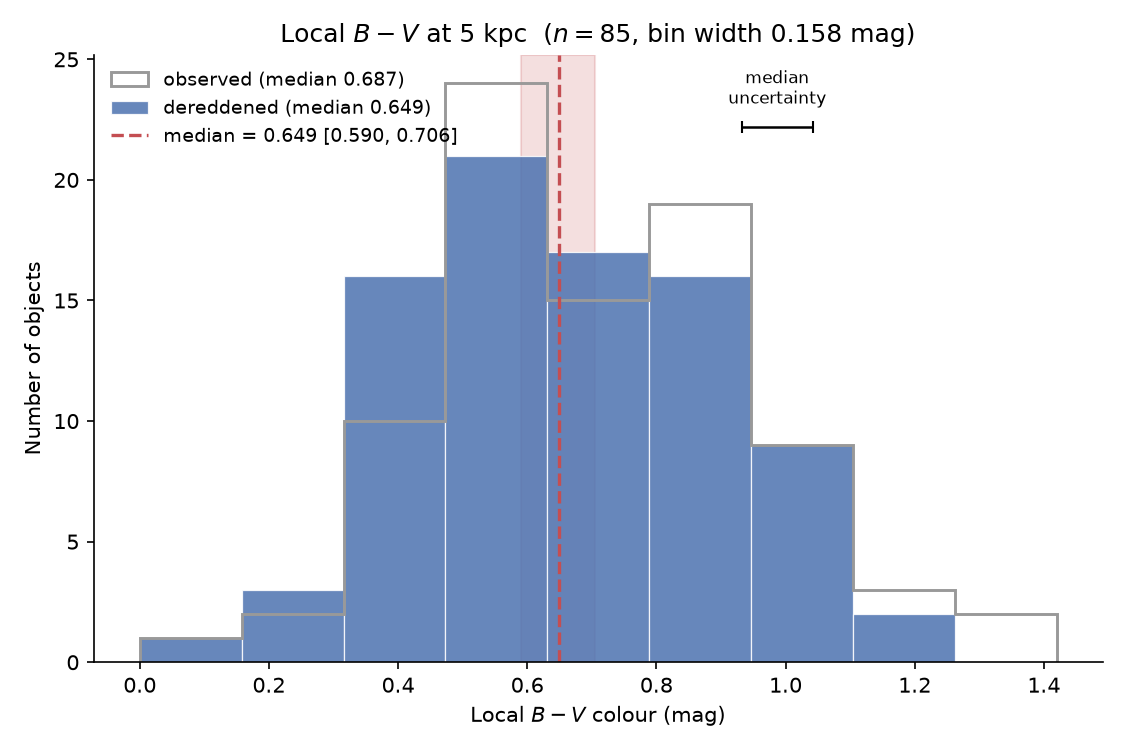
\includegraphics[width=0.8\textwidth]{bv_distribution.png}
\caption{Distribution of calibrated local $B-V$ colour for the final working sample of 98 objects, measured in a 5.0~kpc aperture. The dashed line marks the sample median.}
\label{fig:bv_distribution}
\end{figure}

\begin{figure}[h]
\centering

\includegraphics[width=0.8\textwidth]{color_scatter_paired_bootstrap.png}
\caption{Robust scatter (median absolute deviation) in instrumental local $B-V$ colour across the sample as a function of aperture radius, with a paired-bootstrap 16th--84th percentile band (1000 resamples). Radii marked in red are statistically significantly worse than the 6.5~kpc reference (paired bootstrap difference excludes zero).}
\label{fig:aperture_scatter}
\end{figure}

\section{Discussion}
\label{sec:discussion}

\subsection{The aperture radius result in the context of Kelsey et al. (2021)}

The most notable methodological result of this work is that the radius range found to have significantly elevated local-colour scatter, approximately 1.5--4.5~kpc, brackets the 4~kpc fiducial aperture adopted by \citet{Kelsey2021} for their local $U-R$ measurement. Several factors distinguish the two analyses sufficiently that this should not be read as a direct challenge to their choice: the colour baseline differs ($B-V$ against rest-frame $U-R$, which trace different combinations of stellar age and dust), the host sample spans a markedly different and much lower redshift range (Section~\ref{sec:redshift_compilation}), and the scatter measurement presented here uses instrumental rather than fully calibrated colour. On this last point, however, there is a specific reason to expect the result to be robust to calibration: the zero-point correction applied in Section~\ref{sec:zeropoint_calibration} is an additive constant per image, common to every aperture radius measured for a given object, and is not expected to alter which radius minimises colour scatter across the sample. The result is therefore reported as a genuine, if preliminary, tension worth further investigation with a larger and more thoroughly calibrated sample, rather than as evidence against the appropriateness of a 4~kpc aperture for the different sample and colour baseline used by \citet{Kelsey2021}.

\subsection{Limitations}

Several limitations of the current analysis are worth stating explicitly rather than leaving implicit. First, the uncertainty quoted on each calibrated colour (Section~\ref{sec:zeropoint_calibration}) propagates only the photometric zero-point uncertainty; a photon-noise contribution from the source flux itself has not yet been derived, so quoted uncertainties should be treated as a lower bound on the true measurement uncertainty. Second, the minimum-flux quality cut used to remove implausible colour outliers (a threshold of 1000 counts in either band) is a heuristic identified by inspecting the most extreme resulting colours, not a formally derived signal-to-noise threshold; a complete treatment would incorporate detector gain and read noise, neither of which has yet been extracted from the available image headers. Third, and most fundamentally, one of the two open questions raised early in this project (Section~\ref{sec:imaging_data}) remains unresolved: whether the combined image stacks used throughout this analysis are genuinely free of light from the supernova itself. If SN light were present in some fraction of the stacks, the local photometry presented here would to some degree reflect a mixture of host-galaxy and transient light rather than the host alone, which would not invalidate the aperture-design methodology but would affect the interpretation of the resulting colours. This should be regarded as an open item for supervisor confirmation before the results presented here are treated as final.

Finally, the sample of 98 objects represents a substantial reduction from the 338-object starting catalogue (Table~\ref{tab:final_sample_cuts}), driven primarily by redshift resolution and zero-point coverage rather than by any property of the local colour measurement itself. Given the multi-stage nature of these cuts, the final sample should not be assumed to be an unbiased subset of the parent CSP-I/II sample without further examination; a comparison of the redshift, host type, or light-curve properties of the retained sample against the full catalogue was outside the scope of this work.

\section{Conclusion}
\label{sec:conclusion}

This work has extended the local aperture photometry methodology of \citet{Kelsey2021} from rest-frame $U-R$ colour to observer-frame $B-V$ colour, applied to Type~Ia supernova host galaxies imaged by the Carnegie Supernova Project. A complete pipeline was built from CSP imaging through to a calibrated local colour measurement: photometric redshifts were compiled for 266 of 338 objects via NED; the point-spread function was characterised empirically per telescope and filter, since this sample lacks the uniform seeing selection available to \citet{Kelsey2021}; supernova sky positions were obtained automatically via NED and verified to correspond to the transient site rather than the host nucleus; and a fiducial local aperture radius of 5.0~kpc was justified statistically, via a paired-bootstrap analysis of local colour scatter across the sample, rather than adopted directly from the literature.

The resulting measurement, a calibrated local $B-V$ colour for 98 SN~Ia host galaxies with a median of 0.73~mag, represents a working local-colour catalogue for this sample and a first B-band extension of the Kelsey et al. methodology. The aperture-radius result itself, indicating elevated colour scatter in the 1.5--4.5~kpc range relative to a broader low-scatter plateau from 5--10~kpc, is a genuine finding of this analysis and is discussed above in the context of its limitations.

Remaining work identified over the course of this project includes: resolving whether the CSP image stacks used here are free of supernova light, which bears directly on the interpretation of the measured colours; incorporating a formal photon-noise error budget; and, time permitting, extending the analysis to compare local host colour against SN~Ia light-curve shape and colour parameters, for which a suitable external data source (Uddin et al. 2024, SNooPy light-curve fits for the combined CSP-I/II sample) has been identified but not yet incorporated.


\begin{thebibliography}{9}

\bibitem[Hamuy et al.(2006)]{Hamuy2006}
Hamuy, M., et al. 2006, PASP, 118, 2

\bibitem[Kelsey et al.(2021)]{Kelsey2021}
Kelsey, L., et al. 2021, MNRAS, 501, 4861

\bibitem[Phillips et al.(2019)]{Phillips2019}
Phillips, M. M., Contreras, C., Hsiao, E. Y., et al. 2019, PASP, 131, 014001

\bibitem[Bradley et al.(2019)]{Bradley2019}
Bradley, L., et al. 2019, astropy/photutils, Zenodo, \url{http://doi.org/10.5281/zenodo.2533376}

\bibitem[Astropy Collaboration(2013)]{astropy2013}
Astropy Collaboration, et al. 2013, A\&A, 558, A33

\end{thebibliography}

\end{document}